
%\documentclass[mathserif]{beamer}
\documentclass[handout]{beamer}
%\usetheme{Goettingen}
\usetheme{Warsaw}
%\usetheme{Singapore}



%\usetheme{Frankfurt}
%\usetheme{Copenhagen}
%\usetheme{Szeged}
%\usetheme{Montpellier}
%\usetheme{CambridgeUS}
%\usecolortheme{}
%\setbeamercovered{transparent}
\usepackage[english, activeacute]{babel}
\usepackage[utf8]{inputenc}
\usepackage{amsmath, amssymb}
\usepackage{dsfont}
\usepackage{graphics}
\usepackage{cases}
\usepackage{graphicx}
\usepackage{pgf}
\usepackage{epsfig}
\usepackage{amssymb}
\usepackage{multirow}	
\usepackage{amstext}
\usepackage[ruled,vlined,lined]{algorithm2e}
\usepackage{amsmath}
\usepackage{epic}
\usepackage{epsfig}
\usepackage{fontenc}
\usepackage{framed,color}
\usepackage{palatino, url, multicol}
%\algsetup{indent=2em}
\newcommand{\factorial}{\ensuremath{\mbox{\sc Factorial}}}
\newcommand{\BIGOP}[1]{\mathop{\mathchoice%
{\raise-0.22em\hbox{\huge $#1$}}%
{\raise-0.05em\hbox{\Large $#1$}}{\hbox{\large $#1$}}{#1}}}
\newcommand{\bigtimes}{\BIGOP{\times}}
\vspace{-0.5cm}
\title{Tackling fairness, change and polysemy in word embeddings}
\vspace{-0.5cm}
\author[Felipe Bravo Márquez]{\footnotesize
%\author{\footnotesize  
 \textcolor[rgb]{0.00,0.00,1.00}{Felipe Bravo-Marquez}} 
  
 
%\vspace{-0.3cm}
\institute{Department of Computer Science, University of Chile \\ National Center for Artificial Intelligence Research \\ Millenium Institute Foundational Research on Data }

\titlegraphic{
\includegraphics[scale=0.06]{pics/logodcc.png}
\includegraphics[scale=0.02]{pics/cenialogo.jpg} 
\includegraphics[scale=0.4]{pics/imfdlogo.png}
\includegraphics[scale=0.15]{pics/RELELA.png}}



\date{\today}

\begin{document}
\begin{frame}
\titlepage


\end{frame}


\begin{frame}{Word Vectors}
\begin{scriptsize}
\begin{itemize}
\item A major component in neural networks for language is the use of an embedding
layer.
\item A mapping of discrete symbols to continuous vectors.
\item  When embedding words, they transform from being isolated distinct symbols into mathematical
objects that can be operated on.
\item Distance between vectors can be equated to distance between words.
\item This makes easier to generalize the behavior from one word to another.
\end{itemize}
\end{scriptsize}
\end{frame}


\begin{frame}{Distributional Vectors}
\begin{scriptsize}
\begin{itemize}
\item \textbf{Distributional Hypothesis}: words occurring in the same \textbf{contexts} tend to have similar meanings.
\item Or equivalently: ``a word is characterized by the \textbf{company} it keeps".
\item In this talk we summarize our research addressing three limitations of static word embeddings: 1) fairness, 2) semantic change, and 3) polysemy.

\end{itemize}
\end{scriptsize}
\end{frame}


\begin{frame}{PolyLM: a polysemous language model}
\begin{scriptsize}
\begin{itemize}
 \item A language model capable of automatically learning multiple meanings of a word (e.g. apple:apple, apple:company) \cite{ansell2021polylm}.
\end{itemize}
  \begin{figure}[h]
        	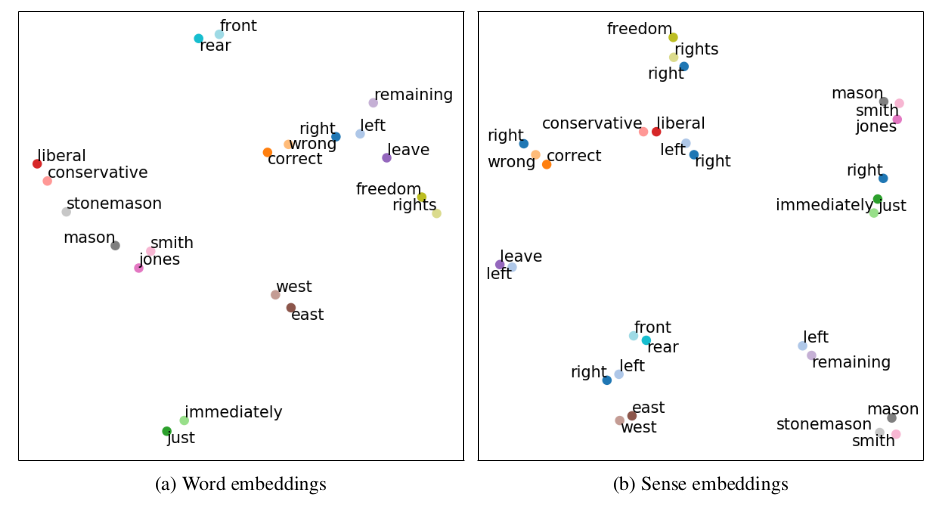
\includegraphics[scale = 0.3]{pics/senseembeddings.png}
        \end{figure}

\end{scriptsize}
\end{frame}



\begin{frame}{PolyLM: a polysemous language model}

  \begin{figure}[h]
        	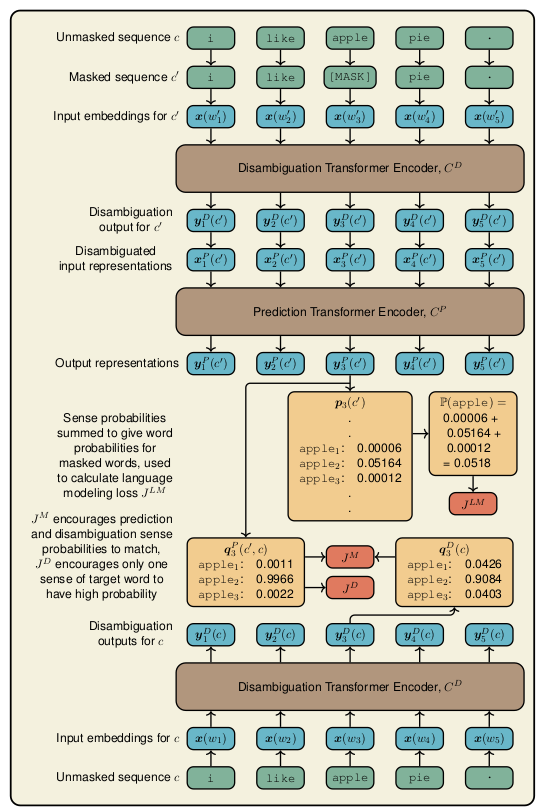
\includegraphics[scale = 0.25]{pics/polylm.png}
        \end{figure}


\end{frame}


\begin{frame}{WEFE: The Word Embeddings Fairness Evaluation Framework}
\begin{scriptsize}
\begin{itemize}
 \item The Word Embeddings Fairness Evaluation (WEFE) is a framework for measuring and mitigating bias in word embeddings (e.g. man is to programmer as woman is to housewife). \cite{badilla2020wefe}.
\end{itemize}
  \begin{figure}[h]
        	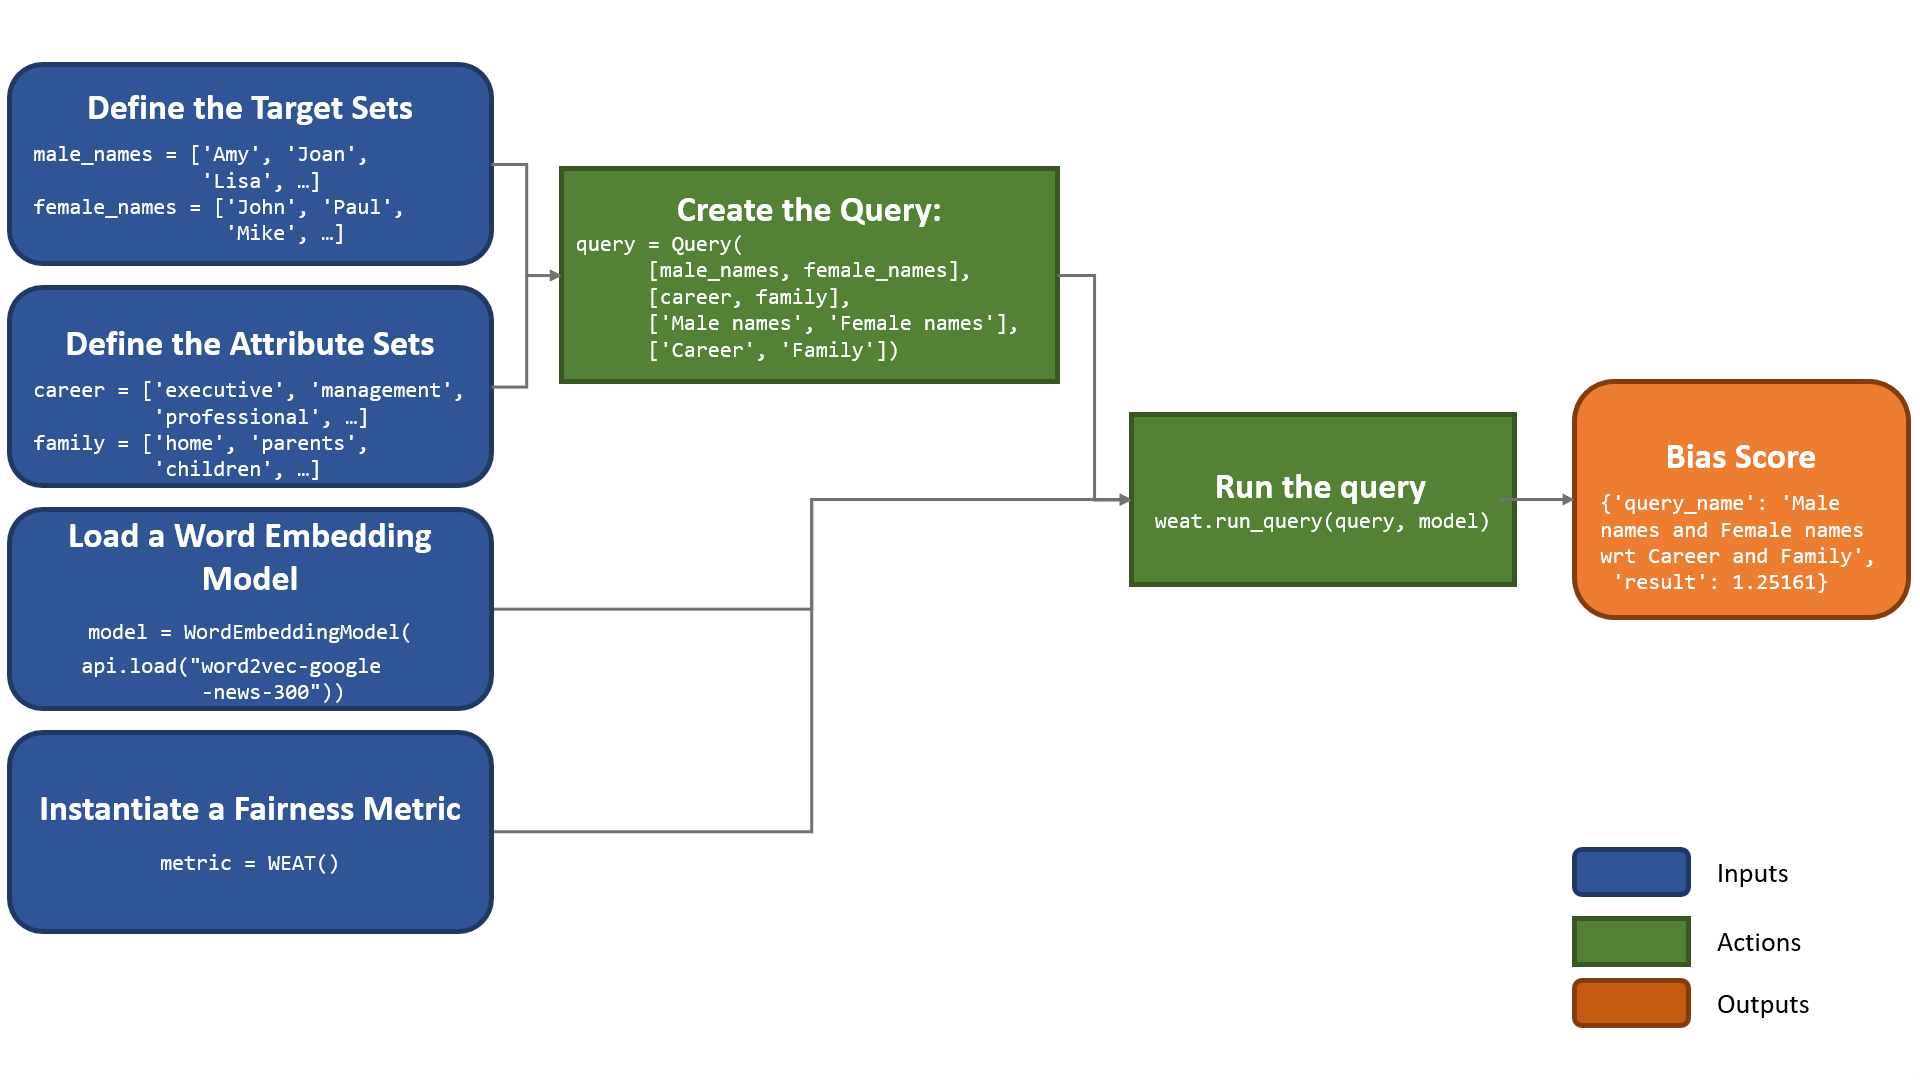
\includegraphics[scale = 0.2]{pics/wefedia.png}
        \end{figure}

\end{scriptsize}
\end{frame}



\begin{frame}{Incremental Word Vectors}
\begin{scriptsize}
\begin{itemize}
 \item An algorithm capable of continuously learning word vectors and thus understanding how the meaning evolves over time (e.g., monitoring the word ``estallido'' in social networks during the Chilean social unrest). \cite{bravo2021incremental}.
\end{itemize}
  \begin{figure}[h]
        	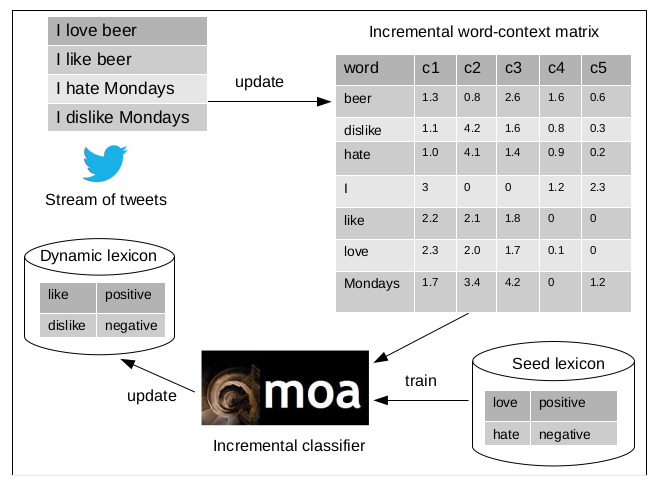
\includegraphics[scale = 0.35]{pics/incdiagram.png}
        \end{figure}

\end{scriptsize}
\end{frame}

\begin{frame}{Incremental Word Vectors}
\begin{scriptsize}
\begin{itemize}
 \item We simulate sentiment change by randomly picking some words and swapping their context with the context of words exhibiting the opposite sentiment.

   \begin{figure}[h]
        	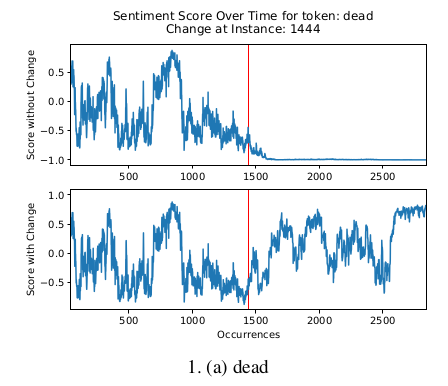
\includegraphics[scale = 0.35]{pics/change.png}
        \end{figure}

 \item Our approach allows for successfully tracking of the sentiment of words over time even when drastic change is induced.

\end{itemize}


\end{scriptsize}
\end{frame}

\begin{frame}
\frametitle{Questions?}
%\vspace{1.5cm}
\begin{center}\LARGE Thanks for your Attention!\\ \end{center}



\end{frame}

\begin{frame}[allowframebreaks]\scriptsize
\frametitle{References}
\bibliography{bio}
\bibliographystyle{apalike}
%\bibliographystyle{flexbib}
\end{frame}  


%%%%%%%%%%%%%%%%%%%%%%%%%%%

\end{document}
